\maketitle
\begin{center}
\huge Work in Progress
\end{center}
\section{Abstract}
Convolutional Neural Networks can be repurposed from their original use case to deliver impressive fingerprint presentation attack-detection accuracy.
This paper explores various options of publicly available machine learning algorithms and transfers their images classifications to differentiate between bona fide and artificial fingerprints.
All networks have their potential evaluated without intrusive modification and after minimal training.

\medskip\noindent
Datasets from the Liveness Detection Competition 2017 were used as training and validation input to give context to the research and compare the results to specialized solutions.


\section{Introduction}
Among all features of the human body, many can be used to authenticate and authorize people by making use of the incredible natural diversity in human appearances. 
Fingerprints in particular have stood out as one of the most reliable method to identify individuals.
Increased availability and compactness of modern digital capture systems have long surpassed analog methods by speed and deliver results quick enough for every day usage.

With all these benefits some problems such as unsupervised misauthorizations can have catastrophic outcomes.
Malicious intent is often connected to high-value targets like critical infrastructure or border control systems, and successful intrusions can lead to severe consequences.
These authentication systems are operating with a high accuracy with no tolerance for errors, which requires highly specialized and costly hardware.
The expensive components make it difficult to integrate high quality fingerprint scanners into systems that are less critical, but still represent attractive targets for unauthorized access like smartphones and personal computers.

Restricted space and aggressive cost optimization create the need for small capture devices which are easy to use, easy to integrate and cheap to produce. 
The reduction in capture-device quality naturally comes with a reduction of authentication accuracy.
Software enhanced authentication systems can deliver impressive results while not requiring complex capture devices.


\subsection{Dataset}
The provided fingerprint samples were originally used as input material for a conference and competition about fingerprint detection. Various materials were used to present a print resembling a finger. 

\smallskip\noindent
About half (45\%) of the dataset are bona fide fingerprints which leaves the other half comprised of the following materials: Gelatine (18\%), Latex(18\%) and Liquid Ecoflex(18\%). 59\% of fingerprint samples are from female subject while 41\% are from males.

\begin{figure}[!htb]
    \centering
    \begin{minipage}[c]{0.15\textwidth}
        \includegraphics[width=\linewidth]{live.bmp}
        \caption{Bona Fide Fingerprint}\label{fig:finger-live}
    \end{minipage}
    \begin{minipage}[c]{0.15\textwidth}
        \includegraphics[trim=32 32 32 32,clip,width=\linewidth]{live.bmp}
        \caption{Sweat Glands}\label{fig:finger-live}
    \end{minipage}
    \hspace{10mm}
    \begin{minipage}[c]{0.15\textwidth}
        \includegraphics[width=\linewidth]{fake-gelatine.bmp}
        \caption{Gelatine}\label{fig:finger-gelatine}
    \end{minipage}
    \begin{minipage}[c]{0.15\textwidth}
        \includegraphics[width=\linewidth]{fake-latex.bmp}
        \caption{Latex}\label{fig:finger-latex}
    \end{minipage}
    \begin{minipage}[c]{0.15\textwidth}
        \includegraphics[width=\linewidth]{fake-ecoflex.bmp}
        \caption{Liquid-Ecoflex}\label{fig:finger-ecoflex}
        \label{img:ecoflex}
    \end{minipage}
\end{figure}

\noindent
All images were captured on a Green Bit DactyScan84C and have a resolution of 500x500px.
The scanner is a standalone high-end device able to capture the fingerprints in high resolution and keeping important details intact.
Bona fide fingerprint images are of such high quality that sweat glands are visible in some samples.

\begin{wrapfigure}[5]{r}{0.5\textwidth}
    \vspace{-4mm}
    \begin{tikzpicture}
    \begin{axis}[
        height=25mm,
        width=95mm,
        yticklabels={},
        xtick={21, 25, 31.3, 40, 77},
        xticklabels={21, 25, 31.3, 40, 77}]

        \addplot+ [
            boxplot prepared={
                lower whisker=19.0, 
                lower quartile=21.0,                
                median=25.0,
                upper quartile=40.0,
                upper whisker=77.0,
                average=31.3
            }
        ] coordinates {};
    \end{axis}
\end{tikzpicture}%
\vspace{-4mm}
\caption{Figure: Age Distribution}
\label{img:age-dist}
\end{wrapfigure}%
%
\smallskip\noindent
The dataset was already split into training and test set with the majority of samples dedicated for validation (37\% training, 63\% testing).

\medskip
\subsection{Neural Networks}
Open-Source libraries like Keras offer simple interfaces for complicated software frameworks like Tensorflow and provide ready-to-use machine learning implementations.
A selection of pre-trained convolutional neural networks was used to conduct the following experiments.

\medskip\noindent
Spacial diversity was a category for selecting the algorithms to provide an insight on how complicated a deep-learning network needs to be in order to provide confident decisions on whether a presented fingerprint image is coming from a live person or not.
It is important to note that these networks were meant to be image classifiers detecting the image's contents.
The classifier MobileNet for example, can detect real world objects and animals and is intended for "mobile and embedded vision applications" (cite MobileNets).

\begin{wrapfigure}[13]{r}{7cm}
    \begin{tabular}{| l | r | r |}
    \hline
    Network Name   & Size    & Parameters \\ \hline\hline
    MobileNet      & 16 MB   &   4,253,864 \\ \hline
    NASNetMobile   & 23 MB   &   5,326,716 \\ \hline
    EfficientNetB0 & 29 MB   &   5,330,571 \\ \hline\hline
 
    Xception       & 88 MB   &  22,910,480 \\ \hline
    InceptionV3    & 92 MB   &  23,851,784 \\ \hline
    EfficientNetB5 & 118 MB  &  30,562,527 \\ \hline\hline

    NASNetLarge    & 343 MB  &  88,949,818 \\ \hline
    VGG16          & 528 MB  & 138,357,544 \\ \hline
    VGG19          & 549 MB  & 143,667,240 \\ \hline
\end{tabular}
\caption{Table: Neural Networks}
    \label{tbl:nerual_networks}
\end{wrapfigure}
\noindent
A total of nine different neural networks were categorized by their size and depth into three groups (see Table \ref{tbl:nerual_networks}).
Each network was custom fitted into the task at hand with wrapper-layer encapsulating the original behavior in a non-intrusive way to ensure that the default behavior is sustained.

\smallskip\noindent
The original input layer was discarded and replaced with a generic Input Layer accepting images of size 250x250. All models share the same input layer implementation.
Furthermore, two additional layers were added to the other end of the stack to flatten the neural network's output and to result in a liveliness score between $0$ and $1$.
Sigmoid is used as the activation function.

\noindent
Each neural networks internal behavior is treated like a black box.


\subsection{Data Acquisition}
\begin{wrapfigure}[13]{r}{10cm}
    \begin{tikzpicture} 
    \begin{umlcomponent}[x=-3,y=0]{Keras} \end{umlcomponent}
    \begin{umlcomponent}[x=3,y=0]{TensorFlow} \end{umlcomponent}

    \umlassemblyconnector[interface=Low Level API]{Keras}{TensorFlow}

    \begin{umlcomponent}[x=2,y=-3]{cnnpad}
        \umlsimpleclass{CnnWrapper}
    \end{umlcomponent}
    
    \umlVHVassemblyconnector[interface=CNN Model Abstractions]{cnnpad}{Keras}


    \umlprovidedinterface[interface=CLI,distance=3cm, with port]{cnnpad}
\end{tikzpicture}
\end{wrapfigure}
Keras is an open-source framework for neural networks and machine learning for the programming language Python.
It offers a simple interface to complex calculations, sophisticated computational resource management and is built on top of TensorFlow (indircite https://keras.io/).

LOOK  HERE Various Python scripts are created for each sequence of the experiment.
Training the networks, saving the trained weights and evaluating the results is done by one pipeline.
Another set of scripts reevaluates best-case trained models and refines the data into human friendly structures.




\subsection{Methodology}
The experiment is split into two parts.
During the first phase the best-case (highest average validation accuracy) for each network needs to be determined.
Due to randomized initial values and subsequent variance in training evolution, the resulting validation accuracy can fluctuate to some degree.
Repetitive training and evaluating will give a set of models for each network which can be serialized and stored.

Models are trained using the provided training dataset over four epochs, which delivered the best balance between validation accuracy and training time.

A total of ten trainings for each network will be used as a pool to pick the best performing model.

\noindent
Trained models are not volatile and can be loaded from disk at any time, so using the best case for each is the fairest approach to make sure every network has the best chances.


\medskip\noindent
Further experiments are conducted in the second phase where the best-case models for each network predicts whether a fingerprint presentation is bona fide or an artificially constructed fingerprint replica.
Unlike neural network training, the predictions of the trained model are static and will not change.
The resulting predictions are used to analyze possible correlations between input data and predicted values.

Just like the original paper about the LiveDet2017 competition, the predictions of each algorithm will be classified by assuming that prediction values of at least 0.50 (cite LiveDet2017) suggest a bona fide fingerprint while all lower values suggest a presentation attack.



\section{Experiment}
\subsection{Phase 1 - Training}

Each network was trained ten times over the course of multiple hours resulting in a representatively distributed set of trained networks.

\begin{wrapfigure}[10]{r}{10cm}
    \vspace{-10mm} 
    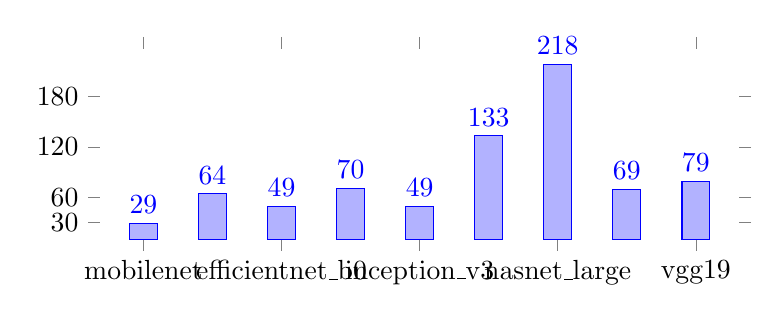
\begin{tikzpicture}
  \begin{axis}[ybar,
        width=100mm, height=40mm,
        x axis line style = { opacity = 0 },
        symbolic x coords = {mobilenet, nasnet\_mobile, efficientnet\_b0, xception, inception\_v3, efficientnet\_b5, nasnet\_large, vgg16, vgg19},
        ytick={30,60,120,180,240},
        nodes near coords,
    ]
    \addplot coordinates { 
        (mobilenet,         29)
        (nasnet\_mobile,    64)
        (efficientnet\_b0,  49)
        (xception,          70)
        (inception\_v3,     49)
        (efficientnet\_b5, 133)
        (nasnet\_large,    218)
        (vgg16,             69)
        (vgg19,             79)
    };
  \end{axis}
\end{tikzpicture}
\vspace{-4mm}
\caption{Figure: Average Training Time in seconds}
\label{img:avg-train-time}



    \vspace{2mm}
    Workstation: Ryzen 2700x (8/16 Cores), 16Gb RAM, GTX 1060 6Gb, TensorFlow Compute Capability: 6.1
\end{wrapfigure}
\smallskip\noindent
The earliest insight is that light-weight, small networks are up to par with bigger, much more complex implementations and that the additional depth of networks like VGG16 is not beneficial for rather simple classifications like presentation attack detection.

\noindent
Surprisingly the most complex network NasNet Large, which also took the longest to train scored the second worst in respect of the median validation accuracy.

\noindent
After the training phase the best-case networks were identified using the average validation accuracy.
The weights for each node are persisted and can be downloaded and applied to reproduce the predictions.
All following analysis will feature these persisted models.


\subsection{Phase 2 - Validation}
Serialized models are loaded and the validation dataset will be interpreted once again while capturing confidence values for further analysis.
The detection error trade-off curve confirms that none of the networks have a clear advantage compared to each other, but shows that NasNet Large and NasNet Mobile performed the worst with an average difference of TBD \% and TBD \% respectively.

\noindent
\begin{minipage}{0.5\textwidth}
    \begin{tikzpicture}
    \begin{axis}[
        width=0.85\linewidth,
        ytick={1,2,3,4,5,6,7,8,9},
        yticklabels={efficientnet\_b0, efficientnet\_b5, inception\_v3, mobilenet, nasnet\_large, nasnet\_mobile, vgg16, vgg19, xception}]
        
        \addplot+ [
            boxplot prepared={
                lower whisker=0.88,
                lower quartile=0.89,
                median=0.89,
                upper quartile=0.88,
                upper whisker=0.91,
                average=0.89
            }
        ] coordinates {};
        
        \addplot+ [
            boxplot prepared={
                lower whisker=0.81,
                lower quartile=0.90,
                median=0.88,
                upper quartile=0.87,
                upper whisker=0.90,
                average=0.88
            }
        ] coordinates {};
        
        \addplot+ [
            boxplot prepared={
                lower whisker=0.83,
                lower quartile=0.89,
                median=0.89,
                upper quartile=0.88,
                upper whisker=0.89,
                average=0.88
            }
        ] coordinates {};
        
        \addplot+ [
            boxplot prepared={
                lower whisker=0.90,
                lower quartile=0.91,
                median=0.91,
                upper quartile=0.91,
                upper whisker=0.91,
                average=0.91
            }
        ] coordinates {};
        
        \addplot+ [
            boxplot prepared={
                lower whisker=0.67,
                lower quartile=0.78,
                median=0.73,
                upper quartile=0.68,
                upper whisker=0.80,
                average=0.73
            }
        ] coordinates {};
        
        \addplot+ [
            boxplot prepared={
                lower whisker=0.66,
                lower quartile=0.76,
                median=0.75,
                upper quartile=0.73,
                upper whisker=0.77,
                average=0.74
            }
        ] coordinates {};
        
        \addplot+ [
            boxplot prepared={
                lower whisker=0.87,
                lower quartile=0.89,
                median=0.88,
                upper quartile=0.87,
                upper whisker=0.89,
                average=0.88
            }
        ] coordinates {};
        
        \addplot+ [
            boxplot prepared={
                lower whisker=0.88,
                lower quartile=0.90,
                median=0.89,
                upper quartile=0.88,
                upper whisker=0.90,
                average=0.89
            }
        ] coordinates {};
        
        \addplot+ [
            boxplot prepared={
                lower whisker=0.86,
                lower quartile=0.88,
                median=0.87,
                upper quartile=0.87,
                upper whisker=0.89,
                average=0.88
            }
        ] coordinates {};
        
    \end{axis}
\end{tikzpicture}
\end{minipage}%
\begin{minipage}{0.5\textwidth}
    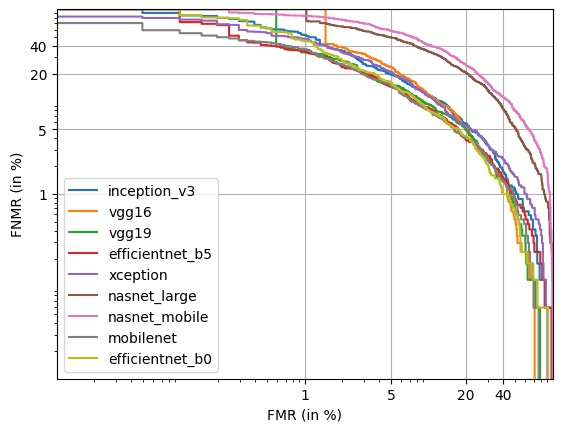
\includegraphics[width=\linewidth]{det-all.jpg}
\end{minipage}


\smallskip\noindent
In the following subsections each network will be inspected individually by evaluating the performance implicitly assuming a neutral FNMR and FMR rate balancing false positives and false negatives.
This allows the performance to be differentiated in terms of certain materials.


\bigskip
\subsection{MobileNet}
\begin{minipage}[c]{0.7\textwidth}
    Bona fide fingerprints were correctly detected with an accuracy of 89.1\%, while presentation attacks were detected correctly with 93.19\%.
    None of the materials show significant variance from each other and are withing a range of 92.0\% and 94.7\%.
    Liquid Ecoflex shows the worst deception potential.

    \medskip\noindent\centering Match Rates: 
    \begin{tabular}{ r  r  r  r |}
        CMR     & CNMR          & FNMR                 & FMR    \\
        89.11\% & 93.19\%       & 6.81\%               & 10.89\% \\
    \end{tabular} \hspace{2mm} Accuracy: 91.33\%
\end{minipage}
\hfill
\begin{minipage}[c]{0.3\textwidth}
    \centering
    \begin{tabular}{ c   r }
    Live               &  89.1\% \\ \hline\hline
    Gelatine\_01       &  92.0\% \\ 
    Latex\_02          &  92.3\% \\
    Latex\_01          &  92.9\% \\
    Gelatine\_02       &  93.5\% \\
    Liquid\_Ecoflex\_01 & 93.5\% \\
    Liquid\_Ecoflex\_02 & 94.7\%
\end{tabular}









\end{minipage}


\bigskip
\subsection{Nasnet Mobile}
\begin{minipage}[c]{0.7\textwidth}

    With a CMR of 81.2\% Nasnet Mobile is the worst performer in the small network group.
    The presentation attack detection for the Latex datasets was with only 63\% slightly better than randomly assigned outcomes.
    A low precision in regards to the materials provide an interesting difference of over 20\% accuracy between Latex and Liquid Ecoflex.

    \medskip\noindent\centering Match Rates: 
    \begin{tabular}{ r  r  r  r |}
        CMR     & CNMR          & FNMR                 & FMR     \\
        81.22\% & 73.97\%       & 26.03\%              & 18.78\%  \\
    \end{tabular} \hspace{2mm} Accuracy: 77.27\%
\end{minipage}
\hfill
\begin{minipage}[c]{0.3\textwidth}
    \centering
    \begin{tabular}{ c   r }
    Live                &  81.2\%  \\ \hline\hline
    Latex\_02           &  63.5\%  \\
    Latex\_01           &  62.9\%  \\
    Liquid\_Ecoflex\_01 &  84.7\%  \\
    Liquid\_Ecoflex\_02 &  86.8\%  \\
    Gelatine\_02        &  75.0\%  \\
    Gelatine\_01        &  70.9\%  \\
\end{tabular}
\end{minipage}



\bigskip
\subsection{EfficientNet B0}
\begin{minipage}[c]{0.7\textwidth}

    The only CMR over 90\% is achieved by EfficientNet B0 which is the second best performer over all.
    Bona fide fingerprints were correctly detected with an accuracy of 92.5\%.
    
    \medskip\noindent\centering Match Rates: 
    \begin{tabular}{ r  r  r  r |}
        CMR     & CNMR          & FNMR                 & FMR     \\
        92.53\% & 88.92\%       & 11.08\%              & 6.23\%  \\
    \end{tabular} \hspace{2mm} Accuracy: 90.56\%
\end{minipage}
\hfill
\begin{minipage}[c]{0.3\textwidth}
    \centering
    \begin{tabular}{ c   r }
    Live               & 92.5\% \\ \hline\hline
    Gelatine\_02       & 85.0\% \\
    Liquid\_Ecoflex\_01& 89.7\% \\
    Latex\_01          & 88.2\% \\
    Latex\_02          & 90.0\% \\
    Liquid\_Ecoflex\_02& 90.0\% \\
    Gelatine\_01       & 90.5\% \\
\end{tabular}









\end{minipage}

\medskip\noindent


\bigskip\bigskip\noindent
Out of the three tested neural networks MobileNet was performing the best on average thanks to it's high true negative detection rate.
The other two networks however have a better true positive rate.
\bigskip\hrule\bigskip


\subsection{Xception}
\begin{minipage}[c]{0.7\textwidth}
    Presentation attack were able to be detected precicely with a max delta of 2.9\% and all accuracies are over 90\%.
    The overall perfoamnce is nothing outstanidng and is in line with the median.

    \medskip\noindent\centering Match Rates: 
    \begin{tabular}{ r  r  r  r |}
        CMR       & CNMR      & FNMR     & FMR     \\
        86.64\%   & 91.47\%   & 8.53\%   & 13.36\%  \\
    \end{tabular} \hspace{2mm} Accuracy: 89.28\%
\end{minipage}
\hfill
\begin{minipage}[c]{0.3\textwidth}
    \centering
    \begin{tabular}{ c   r }
    Live                & 86.6\% \\ \hline\hline
    Liquid\_Ecoflex\_02 & 90.3\% \\
    Latex\_02           & 90.6\% \\
    Latex\_01           & 91.2\% \\
    Gelatine\_02        & 91.5\% \\
    Liquid\_Ecoflex\_01 & 92.1\% \\
    Gelatine\_01        & 93.2\%
\end{tabular}

\end{minipage}


\medskip\noindent


\bigskip
\subsection{Inception V3}
\begin{minipage}[c]{0.7\textwidth}

    The performance is very similar to the previous network with the accuracies differing by only 0.08\%.
    Inception V3s bona fide detection is a little better, but in turn resentation attacks a bit worse in comparison.

    \medskip\noindent\centering Match Rates: 
    \begin{tabular}{ r  r  r  r |}
        CMR       & CNMR      & FNMR     & FMR     \\
        87.76\%   & 90.69\%   & 9.31\%   & 12.24\%  \\
    \end{tabular} \hspace{2mm} Accuracy: 89.36\%

\end{minipage}
\hfill
\begin{minipage}[c]{0.3\textwidth}

    \centering
    \begin{tabular}{ c   r }
    Live                & 87.8\% \\ \hline\hline
    Latex\_01           & 88.8\% \\
    Gelatine\_01        & 89.1\% \\
    Gelatine\_02        & 89.1\% \\
    Liquid\_Ecoflex\_01 & 91.5\% \\
    Latex\_02           & 92.4\% \\
    Liquid\_Ecoflex\_02 & 93.2\% \\
\end{tabular}


\end{minipage}



\bigskip
\subsection{EfficientNet B5}

\begin{minipage}[c]{0.7\textwidth}

    The highest correct non-match rate in the entire series is held by EfficientNet B5 with 96.03\% which is up to par with specialized solutions (cite livdet2017, p7).
    EfficientNet B5 is the best performer on average in the medium size category but the other two networks are very close in accuracy.

    \medskip\noindent\centering Match Rates: 
    \begin{tabular}{ r  r  r  r |}
        CMR       & CNMR      & FNMR     & FMR     \\
        82.70\%   & 96.03\%   & 3.97\%   & 17.30\%  \\
    \end{tabular} \hspace{2mm} Accuracy: 89.97\%

\end{minipage}
\hfill
\begin{minipage}[c]{0.3\textwidth}
    \centering
    \begin{tabular}{ c   r }
    Live                & 82.7\% \\  \hline\hline
    Gelatine\_01        & 94.7\% \\
    Latex\_01           & 95.9\% \\
    Gelatine\_02        & 96.2\% \\
    Liquid\_Ecoflex\_02 & 96.2\% \\
    Liquid\_Ecoflex\_01 & 96.5\% \\
    Latex\_02           & 96.8\% \\
\end{tabular}

\end{minipage}


\bigskip\noindent
Networks in the midrange size deliver as strong performance and are precise in their accuracies.
EfficientNet B5 has the second best accuracy as well as the best CNMR.

\bigskip\hrule\bigskip


\subsection{NASNet Large}

\begin{minipage}[c]{0.7\textwidth}
    More than a fifth of all predictions were incorrect which makes NASNet Large not suitable to enhance the quality of fingerprint presentation attack detection mechanisms.
    With almost 18.2\% of difference between Latex and Liquid Ecoflex, the precision is the worst among all tested networks.

    \medskip\noindent\centering Match Rates: 
    \begin{tabular}{ r  r  r  r |}
        CMR       & CNMR      & FNMR     & FMR     \\
        80.11\%   & 79.41\%   & 20.59\%  & 19.89\%  \\
    \end{tabular} \hspace{2mm} Accuracy: 79.73\%
\end{minipage}
\hfill
\begin{minipage}[t]{0.3\textwidth}
    \centering
    
\begin{tabular}{ c   r }
    Live               &  80.1\% \\ \hline\hline
    Latex\_02           & 70.6\% \\
    Latex\_01           & 71.2\% \\
    Gelatine\_02        & 77.1\% \\
    Gelatine\_01        & 80.9\% \\
    Liquid\_Ecoflex\_02 & 87.9\% \\
    Liquid\_Ecoflex\_01 & 88.8\%
\end{tabular}
\end{minipage}


\bigskip
\subsection{VGG16}
\begin{minipage}[c]{0.7\textwidth}
    The second largest network in this test did not deliver any outstanding data.
    Accuracy and precision are certainly respectable and in the better half of all tested networks, but unremarkable considering the size and prediction latency.

    \medskip\noindent\centering Match Rates: 
    \begin{tabular}{ r  r  r  r |}
        CMR       & CNMR      & FNMR     & FMR     \\
        87.88\%   & 90.29\%   & 9.71\%   & 12.12\%  \\
    \end{tabular} \hspace{2mm} Accuracy: 89.19\%
\end{minipage}
\hfill
\begin{minipage}[c]{0.3\textwidth}
    \centering
    \begin{tabular}{ c   r }
    Live                & 87.9\% \\ \hline\hline
    Latex\_02           & 86.8\% \\    
    Liquid\_Ecoflex\_02 & 88.5\% \\
    Liquid\_Ecoflex\_01 & 89.7\% \\
    Latex\_01           & 91.5\% \\
    Gelatine\_02        & 92.4\% \\
    Gelatine\_01        & 92.9\% \\
\end{tabular}

\end{minipage}



\bigskip
\subsection{VGG19}

\begin{minipage}[c]{0.7\textwidth}
    The largest network provides solid non-match recognition, but cannot provice a good accuracy.
    A CNMR of almost 94\% is the second highest score comparable to algorithms which were handed in for LivDet2017.

    \medskip\noindent\centering Match Rates: 
    \begin{tabular}{ r  r  r  r |}
        CMR       & CNMR      & FNMR     & FMR     \\
        86.93\%   & 93.38\%   & 6.62\%   & 13.07\%  \\
    \end{tabular} \hspace{2mm} Accuracy: 90.45\%
\end{minipage}
\hfill
\begin{minipage}[c]{0.3\textwidth}
    \centering
    \begin{tabular}{ c   r }
    Live                & 86.9\% \\ \hline\hline
    Latex\_02           & 90.6\% \\ 
    Liquid\_Ecoflex\_01 & 92.4\% \\
    Liquid\_Ecoflex\_02 & 93.2\% \\
    Latex\_01           & 93.8\% \\
    Gelatine\_02        & 94.7\% \\
    Gelatine\_01        & 95.6\%
\end{tabular}

\end{minipage}


\bigskip\noindent
Especially with regards to NASNet Large, the additional size seems to provide no benefit to fingerprint presentation attack-detection mechanisms.
For NASNet Large in particular, the additional size does not provide any benefit to fingerprint presentation attack-detection mechanisms.
VGG16 and VGG18 ware both marginally better than the average network and did not deliver the expected accuracy or precision.

\section{Interpretation}
Larger networks suffer from a complex set of layers and nodes that come with no benefits and even weakens the purpose as the increased calculation time brings inconvenience to the potential user.
Predictions may be disturbed with noise coming from convolutional layers providing data which has little-to-no use for fingerprint presentation attack-detection.

\medskip\noindent
The extreme counterexample is MobileNet in this experiment.
An impressive overall accuracy coming from a high CNMR make this convolutional neural network a prime starting point for a competitive alternative.
With only 16Mb in size on disk it is small enough to fit on embedded devices as well.


\section{Conclusion}
Considering the increase in complexity, training and prediction times that deep learning networks with many parameters such as VGG16 bring, the lack in detection accuracy is contrary to expectations.
The original purpose of these networks is to analyze and classify real world objects and animals which bring an acceptable detection rate for fingerprint presentations, but lack the precision and accuracy for real world applications.
With that said, the smaller networks in particular represent a good foundation to fine tune and develop a solution which is better fitting for the job.
By concentrating on the key features of the fingerprint, like the sweat glands or the smooth curvature of ridge lines of the imprint, a much more accurate system can be built.

\medskip\noindent
Image classicfication has many facettes, but the underlying principles are the same for all applications.
Transfer learning is a powerful paradigm that can lead to suprising results when introducing the pretrained models to new use cases.
Given the small training dataset much more accurate predictions are expected when using more extensive reference data to further optimize results.


\section{Bibliography}